\documentclass[10pt,draftclsnofoot,onecolumn,letterpaper]{article}
\usepackage{graphicx}
\usepackage{url}
\usepackage{setspace}

\usepackage{geometry}
\geometry{textheight=9.5in, textwidth=7in}
%\graphicspath{{./images/}}
% 1. Fill in these details
\def \CapstoneTeamName{		Pyranosaurs}
\def \CapstoneTeamNumber{		28}
\def \GroupMemberOne{			Garen Porter}
\def \GroupMemberTwo{			Brooke Weir}
\def \GroupMemberThree{			Alejandro Tovar}
\def \CapstoneProjectName{		OPEnS Pyranometer: IoT Solar Radiation Sensor}
\def \CapstoneSponsorCompany{	Openly Published Environmental Sensing}
\def \CapstoneSponsorPerson{		Chet Udell}

% 2. Uncomment the appropriate line below so that the document type works
\def \DocType{		%Problem Statement
				%Requirements Document
				Design Document
				%Design Document
				%Progress Report
				}
			
\newcommand{\NameSigPair}[1]{\par
\makebox[2.75in][r]{#1} \hfil 	\makebox[3.25in]{\makebox[2.25in]{\hrulefill} \hfill		\makebox[.75in]{\hrulefill}}
\par\vspace{-12pt} \textit{\tiny\noindent
\makebox[2.75in]{} \hfil		\makebox[3.25in]{\makebox[2.25in][r]{Signature} \hfill	\makebox[.75in][r]{Date}}}}
% 3. If the document is not to be signed, uncomment the RENEWcommand below
\renewcommand{\NameSigPair}[1]{#1}

%%%%%%%%%%%%%%%%%%%%%%%%%%%%%%%%%%%%%%%
\begin{document}
\begin{titlepage}
    \pagenumbering{gobble}
    \begin{singlespace}
    	%\includegraphics[height=4cm]{coe_v_spot1}
        \hfill 
        % 4. If you have a logo, use this includegraphics command to put it on the coversheet.
        %\includegraphics[height=4cm]{CompanyLogo}   
        \par\vspace{.2in}
        \centering
        \scshape{
            \huge CS Capstone \DocType \par
            {\large November 27, 2018}\par
            \vspace{.5in}
            \textbf{\Huge\CapstoneProjectName}\par
            \vfill
            {\large Prepared for}\par
            \Huge \CapstoneSponsorCompany\par
            \vspace{5pt}
            {\Large\NameSigPair{\CapstoneSponsorPerson}\par}
            {\large Prepared by }\par
            Group\CapstoneTeamNumber\par
            % 5. comment out the line below this one if you do not wish to name your team
            \CapstoneTeamName\par 
            \vspace{5pt}
            {\Large
                \NameSigPair{\GroupMemberOne}\par
                \NameSigPair{\GroupMemberTwo}\par
                \NameSigPair{\GroupMemberThree}\par
            }
            \vspace{20pt}
        }
        \begin{abstract}
        The wireless, open-source pyranometer project has more to do with hardware than software, thus the design views discussed deal with hardware and physical materials. The project is being sponsored by the OPEnS lab at Oregon State University and there are two stakeholders, Dr. Chad Higgins and Dr. Chet Udell. The pyranometer is to become a part of the environmental sensing collection in the OPEnS lab; it is therefor critical that the pyranometer be able to withstand multiple environments. Most of the physical elements in the pyranometer will relate to weatherproofing or heat regulation in some way and both are crucial in keeping the pyranomator running and reporting accurate data. The pyranometer uses a thermopile to report solar irradiance, so any extra solar energy entering the pyranometer will skew the data. If the data reported by the pyranometer is inaccurate, the pyranometer is rendered useless, thus ensuring accurate data is important part of the design. Each design decision in no way hinders data accuracy, and anything possible is done to potentially increase data accuracy.

        \end{abstract}     
    \end{singlespace}
\end{titlepage}
\newpage
\pagenumbering{arabic}
\tableofcontents
% 7. uncomment this (if applicable). Consider adding a page break.
%\listoffigures
%\listoftables
\clearpage

% 8. now you write!
\section{Introduction}
\subsection{Project Description}
The overall project is a wireless, open-source pyranometer. A pyranometer is a device that detects solar radiation and reports a $W/m^2$ value based on the total amount of solar radiation hitting the device. Open-source pyranometers exist, but they are generally poorly documented and wired. This pyranometer will be easy to set up due to good documentation and will be wireless.
\subsection{Stakeholders}
\subsubsection{Dr. Chet Udell}
Our primary client, Dr. Chet Udell, is the director of the Openly Published Environmental Sensing (OPEnS) lab. The OPEnS lab is the primary sponsor of our project and our pyranometer will become one of the many OPEnS lab wireless sensors.

\subsubsection{Dr. Chad Higgins}
Dr. Chad Higgins is an associate professor in the College of Agricultural Sciences, specically in College of Biological and Ecological Engineering. Dr. Higgins conducts many ecological studies and a pyranometer will be especially helpful for such studies. He will want accurate readings from the pyranometer. 

\subsection{Design and Stakeholder concerns}
The main concerns are cost to build, easiness to build, and accuracy of data. One of the main purposes of the open-source pyranometer is to have it be cheap and easy to build by anyone with access to a 3D printer. Researchers and scientists should be able follow the documentation for the pyranometer and construct it without any headache. The data reported by the pyranometer needs to be reliable, otherwise it is useless. A fourth concern is the pyranometer's surviveability; the pyranometer needs to be weatherproof and the power source needs to last at least a few weeks.

\subsection{Design Viewpoint Descriptions}
\subsubsection{Black Body Object}
The black body object is what the thermopile senses in order to report the total solar radiation hitting the pyranometer. The object is meant the absorb solar radiation and emit IR radiation, which is detected by the thermopile and used to report the total solar radiation hitting the pyranometer.

\subsubsection{Power Source}
The power source is what supplies power the pyranometer. The power supply must be wireless and be able to sustain the pyranometer for weeks at a time.

\subsubsection{Data Transmission}
Data transmission refers to how the pyranometer wirelessly sends data back to the user. It is assumed that the user has a data hub or receiver that the pyranometer sends data to.

\subsubsection{Data Logging}
Data logging is how data from a sensor can be recorded. In this case, it refers to logging data manually for testing sake.

\subsubsection{Housing Structure}
The housing structure is the 3D printed object that will contain all other parts of the pyranometer to make it one sensor. 

\subsubsection{Weatherproofing Housing Structure}
Weatherproofing the housing structure refers to keeping the pyranometer safe from the elements. These include rain, water, and wind. 

\subsubsection{Analog Translation}
Analog translation is the method of converting the data gathered by the sensor in to usable data. For our project, we want the data to be converted into units $W/m^2$.

\subsubsection{Light Diffuser}
The light diffuser will be used to assist the sensor. It will evenly spread light onto the sensor to give consistent and acurate data.

\subsubsection{Dome Structure}
The dome structure is the material used to protect the light diffuser and sensor. It will be transparent to allow light to pass through and needs to meet weatherproofing criteria.

\section{Project Identification}
\subsection{Date}
The pyranometer project was assigned to the group on October 8th, 2018. It will end on the Engineering Expo hosted by Oregon State University in May, 2019. 

\subsection{Scope}
The pyranometer will be able to measure solar radiation and convert it to $W/m^2$. It will then transmit that data to a Google spreadsheet using the LOOM architecture. The goal of this project is to create an open-source and low-cost pyranometer that is comparable to an industry standard.  The project will also be open-source by adding any code added to the LOOM system on GitHub. All of the technology used to create the pyranometer should be available to any other lab or Maker Space. It should be able to be recreated with a 3D printer and access to funds to buy a few low-cost electronics. The benefit of creating something open-source is that it can be built all over the world. This is helpful because measuring solar radiation is good information around the globe. One use for this sensor is to use it for agriculture. Plants need sunlight to survive and using a pyranometer to know how much sunlight a particular area is getting is good information.

\subsection{Issuing Organization}
OPEnS lab is the primary sponsor of the wireless open-source pyranometer project, with Dr. Chad Higgins supplying the idea of the project. Once the project is complete, the pyranometer will become a part of the OPEnS collection of open-soure sensors.

\subsection{Authorship}
The authors and editors of this project are Brooke Weir, Garen Porter, and Alejandro Tovar. Suggestions, guidance, and recommendations made by Dr. Chad higgins and Dr. Chet Udell have influenced design decisions and edits made to most written documents for the pyranometer project. 

\subsection{Context}
There is a need for an open-source pyranometer that is wireless and well documented. Existing open-source pyranometers are either poorly documented or wired, so researchers who are looking for an open-source pyranometer that is well documented and wireless have no options. The wireless open-source pyranometer project will fill this need and look to serve researchers who need a cheap, wireless, and easy to assemble pyranometer. Most wireless pyranometers are expensive, and the open-source nature of this project serves will make the pyranometer much cheaper (only cost of materials and assembly need to be accounted for).

\section{Design Views}
\subsection{Black Body Object: Painted 3D Printed Dome}
Thermopiles, which is what is going to be used to report $W/m^2$ data, is a device that reads the temperature of an object using a die with a known temperature. More precisely, the thermopile reads the IR emanated from an object to calculate the object's temperature. To get accurate readings, black objects with high emissivity values need to be used. 
\subsubsection{Design Concerns}
The first concern is material cost and availability. Ideally, a cheap object with high emissivity should be used. The first material that comes to mind is Teflon, which is cheap and has an emissivity value of 0.92 (fairly high). Teflon, however, leads to the second concern; the object's ability to be shaped and formed. Teflon is a hard plastic that can only be shaped by a laser cutter and is not easily formed into shapes other than a sheet. Thermopiles work best when pointed at an infinite plane, and the best way to implement an infinite plane is to place the thermopile inside a dome, where the dome is the black body object. It may be possible to form Teflon into a dome shape, but it would be exceedingly difficult. An alternative, and what is now perceived as the best option, is to 3D print a dome out of Polyactic Acid (PLA) and paint the dome with Black 2.0. PLA is a popular plastic in 3D printing and its surface is able to be painted. PLA is inexpensive and 3D printing a dome structure will be easy and the dome can be made with any desired dimensions. Black 2.0 is the blackest and mattest paint available for purchase. A tube is about \$20 and will make the emissivity of the PLA about 0.99.\\A third concern is the accuracy of the data; which is directly related to the emissivty of the black body. The higher the emissivity of the object the higher the accuracy of the data. The emissivity of black PLA is about 0.92, but when the PLA is coated with Black 2.0 the emissivity increases. The emissivity of PLA by itself is high enough to where a user would not \textit{have} to paint it, but it would be best if users did use Black 2.0 to paint the PLA.
\subsubsection{Design Elements}
There are three required elements for the optical black object; a coil of black PLA; a 3D printer; a tube of Black 2.0; and a CAD design of the dome. The CAD file will be used to tell the 3D how to construct the dome. Once the dome is finished printing, it must be painted with Black 2.0 to achieve the highest emissivity possible. There needs to be a small slit on one side of the dome that allows the wires coming from the thermopile to pass under. The dome will be glued to the base of the housing structure with the thermopile inside. The dome should simulate an infinite black plane that allows the thermopile to get the most accurate readings possible. 
\subsubsection{Design Relationships}
The black object directly effects the thermopile and the housing structure. The dome is glued to the base of the housing structure and it must fully encapsulate the thermopile. The optical black object is a crucial element in ensuring accurate data is read from the thermopile.
\subsubsection{Design Rationale}
Ideally, an infinite plane with an emissivity value of 1 would be used as the optical black object. A dome surrounding the thermopile will accurately simulate an infinite plane, and coating black PLA with Black 2.0 will give as high an emissivity value as possible at a reasonable price. This approach to the optical black object should result in the most accurate data readings possible.

\subsection{Power Source}
A large part of this pyranometer project is to make it wireless, which primarily means that the pyranometer must have a wireless power source. There are several different possible routes to go, and different users may have different preferences. For the OPEnS open-source pyranometer, lithium batteries will be used, but the documentation will mention possible alternatives (solar panel, generators, etc.). 
\subsubsection{Design Concerns}
The main concern with the power source is how long it will last. The power source itself is the main factor in battery life, but the efficiency of the code in the microcontroller and how many sensors are connected to the microcontroller must also be considered. The current design has two thermopiles and a LoRa radio chip being connected to the Feather M0 microcontroller. All three of these take little power. LoRa is not power intensive by nature, and the thermopile sensors take readings every few seconds and are put in a low power state between taking readings.\\It was decided that lithium-ion batteries would be used to power the pyranometer. An initial concern was ease of use, and it is very easy to hook up a lithium batter pack to a Feather M0 (as simple as plugging a wire into a pin). Other implementations, such as a solar panel or thermoelectric generator, had a much more involved setup. The OPEnS lab already has lithium battery packs purchased, so no additional money needs to be spent on lithium batteries. For users outside the lab, the battery packs will cost between \$50 and \$75 dollars, but they are rechargeable and should last several weeks or months. There is a large discrepancy between the low end and high end of the estimated life of the batteries. This is due to the code efficiency playing a large role in how long the batteries will last, and it is difficult test the code's effect on the battery without deploying the pyranometer to the field and timing how long it lasts. 
\subsubsection{Design Elements}
For the power source there is only one design element, and that is the battery pack itself. The pack that OPEnS lab uses is a collection of six "AA size" lithium batteries. Other OPEnS projects reportedly last a couple months per charge, but it varies depending how well the code is written and how many sensors are a part of each project. The batteries are rechargeable and have a relatively low discharge rate (meaning not much charge capacity is lost per recharge) and can be recharged a few hundred times before needing to be replaced. 
\subsubsection{Design Relationships}
The project as a whole will not work without a power source, but the power source itself only effects the Feather M0 microcontroller and the housing structure. The housing structure needs to adequately protect the lithium batteries from any form of weather, and any heat coming from the batteries needs to be isolated from the optical black object. This entails the lithium batteries being enclosed by walls. The power source needs to adequately supply power the Feather M0 so that it may perform its functions for long periods. As long as the lithium batteries keep the Feather M0 running for long periods of time and the lithium batteries are adequately protected; the batteries are performing their job.
\subsubsection{Design Rationale}
Various power sources were judged based on three criterion; cost, ease of use, and average life. Lithium batteries are expensive initially, but can be reused over and over, so the overall cost is relatively low. Lithium batteries are long lasting in two senses; each charge of a lithium battery pack lasts a long time and the batteries can be reused over and over giving them a long overall life. Finally, lithium batteries are easy to use; simply plug them into the Feather M0 to power it, and plug them into a charging station to charge them. The pyranometer documentation will recommend a battery pack to buy, so users should be able to order the batteries and begin using them immediately. The housing structure will have an enclosure to set the battery pack in, with the goal of the enclosure being minimizing the heat impact of the batteries. The ease of use, longevity, and value of lithium batteries make them the ideal design choice for the pyranometer project.

\subsection{Data Transmission: LoRa Radio}
The purpose of using LoRa radio with the pyranometer is to wirelessly transmit data over long distances. LoRa is a wireless communication technology that consumes low amounts of power while being able to transmit data or long distance; the caveat is that LoRa operates under low bandwidth, thus limiting the amount of data that can be sent.
\subsubsection{Design Concerns}
There are several concerns when implementing LoRa radio, first of which is keeping power consummation low. LoRa, by nature, consumes low amounts of power compared to other data transmission methods (Wifi and Cellular), but to further assist with power consumption the \textit{rocketscream/Low-Power} Arduino library will be used. The library assists with power management by frequently putting the Feather M0 in a lower power mode.\\A second concern is keeping the pyranometer structure weatherproof. Using LoRa radio requires use of an external antennae, which means that an antennae needs to protrude out of the housing structure. To make this protrusion possible, a hole will need to made in the housing structure. The hole will need to be just wide enough to fit the antennae, and a resin will be applied around the hole to help seal the crack between the antennae and the housing structure.\\A third concern is fitting the LoRa transmitter chip neatly inside the housing structure. Within the housing structure, there will be the Feather M0 microcontroller attached to a multiplexer, two thermopile sensors, a lithium battery packet, the LoRa radio chip, and two black body objects. All of the hardware needs to fit inside as small of a structure as possible and not interfere with the readings from the thermopiles. To limit interference, there will need to be a barrier between the black body object and the LoRa chip (any source of external heat will interfere with the black body temperature). The housing structure is going to be 3D printed, so thin 3D printed barriers will be made between each chip, and the LoRa radio chip will be placed on the edge of the inside of the structure. An SMA connector will be facing the inside of the outer wall of the structure, thus allowing the antennae to be easily screwed in from the outside. 
\subsubsection{Design Elements}
The physical chip that will be used is an \textit{Adafruit RFM95W LoRa Radio Transceiver} along with a SMA connector to allow an antennae to be securely connected to it. The chip will be connected to a multiplexer that will be connected to a Feather M0 (the microcontroller controlling the pyranometer and making all computations). The chip itself is about the size of a quarter, and the antennae and SMA connector take up no space inside the housing structure.\\The \textit{LOOM LoRa API} will be used to setup and configure the LoRa radio with the pyranometer. The API has implementations for receiving and sending OSC bundles (data packets containing sensor readings). The LOOM LoRa API makes use of the following APIs and libraries: \textit{adafruit RadioHeaad, GreyGnome EnableInterrupt, FabioCuomo FabioCuomo-DS3231, rocketscream Low-Power, CNMAT OSC}, and \textit{EnviroDIY Arduino-SDI-12}. Each library is made specifically for use by Arduino microcontrollers, and each library assists or enhances the LoRa radio implementation. 
\subsubsection{Design Relationships}
The wireless transmission, both the non-physical and physical aspects, relate to the housing structure, black body objects, and Feather M0. The housing structure will need to have a wall between the LoRa chip and the black body object to limit interference. The housing structure will also need a hole cut where the radio antennae needs to poke out of. The Feather M0 will need to be configured to send data packets over LoRa radio to a LoRa receiver. The LOOM API has a configuration file that will need to set to use LoRa. With the configuration file correctly configured, the thermopile readings will need to be organized into OSC packets (this is all done by the API). The only code that will need to be written is a call to the LoRa send function (the function will be called in the main loop every few seconds). 
\subsubsection{Design Rationale}
LoRa radio is the best option for data transmission due to its low power consumption and high range. There is an existing API already implemented in LOOM to make LoRa easy to implement. Many other OPEnS IoT devices usu LoRa as well, so there are LoRa receivers already set up and there are examples to follow. As long as the housing structure is designed carefully, the weatherproofing and data interference concerns can be negated.

\subsection{Data Logging: Adalogger}
LOOM will be used to log data from a sensor onto either a spreadsheet or a micro SD card. When configuring the LOOM system for the pyranometer, LOOM can either put the recorded data on a micro SD card or transmit it to a Google spreadsheet. To upload to a Google spreadsheet, the pyranometer will use LoRa radio which was covered earlier. In this section, the SD card route using the Adafruit Adalogger will be examined. 

\subsubsection{Design Concerns}
The major concern with the Adalogger is that the information recorded on the SD card will have to be manually taken from the sensor and onto a computer. Having to manually move the data will not be helpful for a sensor since they are meant to be left outside for a long period of time without human involvement. Also an SD card can only hold so much data. The SD card will mostly be involved during the testing of the sensors so the concern is valid, but the SD card will not be involved in the final prototype.

\subsubsection{Design Elements}
The Adalogger can be hooked up to a multiplexer that is also connected to the Feather M0 and a sensor. The Adalogger can take the data from the sensor and put it on a micro SD card. The micro SD can then be taken out and put into an SD card. The files on the SD card can then be read from a computer. 

\subsubsection{Design Relationships}
The Adalogger will be connected to the multiplexer and Feather M0. The multiplexer is what connects the sensor to the Feather M0 and Adalogger. The Adalogger will take the data that the sensor gets and put it on a micro SD card. 

\subsubsection{Design Rationale}
The purpose of the Adalogger is to give a quick way to get data from a sensor for testing. Testing is an important part of making sure that the data the pyranometer senses is accurate. Using the Adalogger is a good way to get the data and determine if it is correct. 

\subsection{Housing Structure: A 3D Printed Design}
The housing structure will enclose the electronics for the pyranometer such as the sensors, a LoRa radio chip, and others. It will be 3D printed with a space for an antennae to poke out. 

\subsubsection{Design Concerns}
A concern for the housing structure is to fit all the electronic pieces within the structure while not cramming the electronics too closely. This is important so that the sensors do not pick up heat from other electronics such as the battery pack or LoRa radio chip. The Feather M0, LoRa radio chip, and any other electronics will have to maintain some distance from the black bodies and sensors. Otherwise the data will not be accurate.\\
Another concern is the hole where the LoRa antennae will poke out of the structure. It leaves a space in the housing structure where the elements can affect the electronics more easily. Rain or wind can enter the structure and screw the data as well as create damage. The resin applied to the 3D printed structure should prevent such damage from happening, but the antennae does leave room for error. 

\subsubsection{Design Elements}
The housing structure will be 3D printed and then coated with a resin. To create the structure, CAD will be used to create the design and one of the three 3D printers available at the OPEnS lab will be used to print it. The structure will then be coated in a resin to help weather proof the design. The antennae for the radio will be added to the housing and have a resin applied to minimize the space where the elements can enter the pyranometer. 

\subsubsection{Design Relationships}
The housing structure has a relationship with all other components of the pyranometer since it will contain all of them. All of the parts of the pyranometer, except the radio antennae, will be contained within the housing structure. The radio antennae will be partially enclosed in the structure.

\subsubsection{Design Rationale}
The purpose of the housing structure is to have something to surround all of the electronics so each unit is portable. It is there so that there are not loose electronic pieces. The housing structure also protects the electronics from the elements. The housing structure allows the components to be put together and called one single sensor. 

\subsection{Weatherproofing Housing Structure: 3D Printing and a Resin}
Weatherproofing the housing structure for the pyranometer is important to protect the electronics and to obtain accurate data. The structure itself will be 3D printed with a LoRa radio antennae sticking out of the structure. The structure will have to be protected from the elements as well as insulated to get accurate, reliable data. 

\subsubsection{Design Concerns}
There are several concerns for weatherproofing the housing structure for the pyranometer. The first concern is to prevent water damage on the sensor inside the housing. Water damage can seriously damage the technology. There will be some areas where the possibility of water damage will be higher. One such area is where an antennae will protrude out of the housing structure for the LoRa radio. Preventing water damage is crucial to keep the battery, Feather M0 working, and other electronics working. Another concern with waterproofing the housing structure is to protect the sensors that depend on heat to read data. Heat comes from the sunlight coming in, but also wind and ambient heat affects the temperature. The housing structure should be insulated from wind and other types of heat. 

\subsubsection{Design Elements}
The housing structure will be 3D printed. There are ways to 3D print the housing structure to make it more waterproof. The first way to do so will be to print the thick layers [4]. This will reduce the overall amount of layers which will decrease the areas that water can slip through between layers. The second way to do so will be to print the housing structure will 100\% infill [4]. The third way to do so will be to print several perimeters to enclose the electronics. Having smaller structures enclosed within another structure will add to the number of layers water will have to go through to damage the electronics. It can also help insulate the electronics from wind and heat.\\
Beyond 3D printing the structure in particular ways, another way to weatherproof the housing structure is to apply a resin. Applying a resin to the 3D printed structure will fill in the gaps between the layers. The resin itself will be resistant to the elements and help the overall structure from being damaged. 

\subsubsection{Design Relationships}
Weather proofing the housing structure has a relationship with everything inside the structure. It will have to protect everything inside from wind, rain, and ambient heat or lack thereof. Specifically, weather proofing will interact with the LoRa radio antennae since the antennae will have to protrude outside of the housing structure. Otherwise, the housing structure will protect the Feather M0, two thermopile sensors, a battery, a LoRa radio chip, and two black body objects. 

\subsubsection{Design Rationale}
The purpose of weather proofing the housing structure is to protect the electronics from the elements such as wind, rain, and heat. This is necessary to keep the pyranometer running. Each component, aside from the black body objects, inside the structure will be small electronics. Those pieces will be susceptible to water damage. Protecting against wind and heat will protect the electronics from experiencing extreme temperature fluctuations as well record accurate data.

\subsection{Analog Translation}
Analog Translation is the process of converting solar radiation into some form of usable data. For this project we want to be able to read in solar radiation as $W/m^2$. The micro-controller needs a way to achieve this translation. There are some hardware that can simplify this task, but can be expensive. For our purpose, using open source software and modifying it for our needs will be best suited for this project.
\subsubsection{Design Concerns}
The written and modified code will need to be simplified and well documented for other users to understand. Once we can get our code to compile and translating data, we will need to run tests to determine the accuracy of our translations. The code will also need to be compatible with the chip if the micro-controller and to maker sure we don't overwork the chip with the program.
\subsubsection{Design Elements}
The micro-controller will be programmed with our translator to read in data as heat. Then using a physics equation that will need to be derived, the program should be able to take in the data the micro-controller is reading and convert it into data with units $W/m^2$. The data will then be ready to be sent and logged on a spreadsheet.

\subsubsection{Design Relationships}
The design of this program will be compiled and downloaded onto the chip of the micro-controller to perform it's calculations. It will get the data that was gathered from the sensor and convert it into our desired data in $W/m^2$ units.
\subsubsection{Design Rationale}
Using open source software is better for this project because it is being integrated into an open source data hub. The goal of the project is to get a solar radiation sensor onto the Loom git hub repository for others to use. It is cheaper than having to buy dedicated hardware that can do this translation for us. 

\subsection{Light Diffuser}
The light diffuser is a piece of material that will spread light evenly onto the sensor. This part of the device plays an important role in the accuracy of our sensor. The light transmittance efficiency of the diffuser will play a big role in the design of this part. The light transmittance efficiency is a rating of how much light passes through an object.
\subsubsection{Design Concerns}
Some concerns will be material of the diffuser and the thickness. It needs the right amount of light transmittance.  The sensor is like the human eye, too much light and it will be blinded by bright light, but too little light and it will be difficult to see. We need the right amount of light to pass through our diffuser. We don't want to overstimulate the sensor or not have enough. The material will determine how much light and what kind of light can get through. Thickness will also determine how much light will pass through. Price of the material is also a concern that will need to be taken into account.
\subsubsection{Design Elements}
Our ideal diffuser will have a surface called a Lambertian surface. A Lambertian surface is the ideal surface for diffusing light. The idea is that the brightness of light is the same regardless of the observer's angle view. If our diffuser has this kind of effect, then we can evenly distribute light for an accurate reading. We plan on using our diffuser as both a diffuser and to play small role in protecting our sensor. The diffuser will be dome-like to account for all angles of sunlight.
\subsubsection{Design Relationships}
The diffuser will have to be big enough to cover our sensor. This is to get the most out of the sensor. It will also have to adhere to the housing structure as well. We will have to make sure that this piece maintains our goals of weather proofing the device.
\subsubsection{Design Rationale}
The diffuser needs to be able to distribute light as even as possible to give our sensor enough data. It will also need to let in the right amount of sunlight so the sensor doesn't get overstimulated or have to little to work with. A dome size structure is needed to cover the sensor as well as to fit in the housing structure design. White diffusing glass will be used as it has a good light transmittance that can adjusted by adding layers of glass to increase or decrease thickness.

\subsection{Dome Structure}
The dome structure is what will overall protect the sensor as well as the diffuser. It will need to be durable and be able to let sunlight in. As well as meet the weather proofing goals since it is an outer layer of our device. For the dome structure, the material will be made out of acrylic plastic. 
\subsubsection{Design Concerns}
Some concerns include cost, durability, and light transmittance efficiency. The material used will need to have a low cost to keep our device from being too expensive. The material will also have to be durable to survive long periods of time in any environment it is use in. Since this will cover our diffuser, we need to maker sure light can pass through and enough light passes through to the diffuser. This will play a role in the accuracy of the sensor.
\subsubsection{Design Elements}
The dome structure will be bigger than the diffuser in order to cover and protect it. The material will be acrylic. The dome structure will have the same shape as the diffuser to for this design. 
\subsubsection{Design Relationships}
The dome structure is used to protect the diffuser and the sensor. It will need to fit with the housing structure as well. Since it is a part of the housing structure it will need to be weather proof just like the rest of the structure.
\subsubsection{Design Rationale}
Acrylic material will be used for this dome structure. It is more durable than glass, and less heat conductive. This is important because the sensor will read in heat, and any external heat can lead to errors. Acrylic is also cheaper than other viable materials, making it the better choice in terms of cost. The material also has a high light transmittance and lets in the most amount of different wavelengths of sunlight. The sensor needs to read in UV, Infrared, and the visible spectrum so acrylic is the ideal choice.

\section{Conclusion}
\begin{figure}[h]
\centering
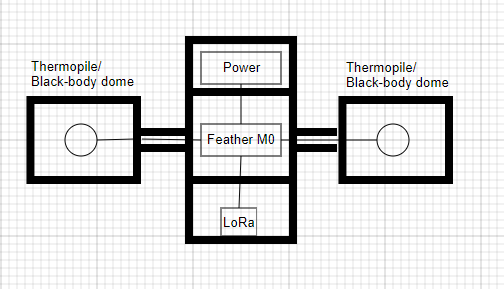
\includegraphics[natwidth=504,natheight=289]{pyro.PNG}
\caption{Top-down design of the open-source pyranometer.}
\end{figure}
Figure 1 shows the current design of the open-source, wireless pyranometer. The design is heavily influenced by various design concerns, such as data accuracy, cost, and ease of assembly. Each hardware piece is put behind a 3D printed wall, and the thermopiles (and surrounding black-body dome) are put behind two walls to limit any excess thermal energy from interfering with the thermopiles' readings. Each wall will have a small slit for wires to go through, but each hardware piece should otherwise be separate from each other. Having different "compartments" for each hardware piece should make assembly easier, as users will simply need to place each hardware piece in its respective slot. The entire structure, as well as the domes surrounding the thermopiles, will be 3D printed to limit cost. A second 3D printed structure will be placed over the top of the base to protect the hardware from the environment in order to keep it weatherproof.\\\\
A common theme throughout the various designs is keeping pyranometer safe in the field (deployed in the environment) and ensuring the data it reports is accurate. All of the OPEnS sensors are meant to live out in various climates and the pyranometer is no different. In each design decision, weatherproofing and data accuracy were considered to help ensure that the pyranometer is reliable in most environments. Besides keeping the pyranometer weatherproof and ensuring accuracy of data, ease of assembly and price are two important factors considered in each design decision. Everything that can be 3D printed is being 3D printed to keep cost down and make assembly easier. For the parts that cannot be 3D printed, such as the top domes, the best value parts are chosen. The design decisions made should lead to a pyranometer that can survive in most environments, be easy to assemble, be inexpensive (relative to other wireless pyranometers), and produce reliable data.

\section{Glossary}
\textbf{Black 2.0}: \textit{The blackest paint available to the public; created by Stuart Semple and inspired by Vantablack [1].}\\\\
\textbf{Emissivity}: \textit{An objects ability to emit thermal radiation (IR).}\\\\
\textbf{Feather M0}: \textit{A small, lightweight microcontroller developed by Adafruit.}\\\\
\textbf{Infrared (IR)}: \textit{A form of electromagnetic radiation emitted from heated objects.}\\\\
\textbf{Lambertian Surface}: \textit{ A quality a transparent object may have. Where the brightness of light passing through is the same in any angle it is viewed at. This is regarded as an ideal diffuser}\\\\
\textbf{Light Diffuser}: \textit{An object that can evenly distribute light passing through on a surface.}\\\\
\textbf{Light Transmittance Efficiency}: \textit{A rating on the percentage of light that can pass through an object.}\\\\
\textbf{Lithium-ion battery}: \textit{A rechargeable battery that generates electricity via the movement of positively charged lithium ions.}\\\\
\textbf{Long Range (LoRa)}: \textit{A wireless communications technology developed by Semtech [2]}\\\\
\textbf{LOOM}: \textit{An IoT system designed by the OPEnS lab. It seeks to make the process of creating IoT devices simple.}\\\\
\textbf{Pyranometer}: \textit{A device that detects solar radiation and reports the total solar irradiance in $W/m^2$.}\\\\
\textbf{Open-source}: \textit{Refers to software and code being freely available to the general public.}\\\\
\textbf{Openly Published Environmental Sensing (OPEnS)}: \textit{An organization sponsored by Oregon State University dedicated to creating open-source environmental sensors using modern technology.}\\\\
\textbf{Resin}: \textit{A material that is insoluable to water.}\\\\
\textbf{SD card}: \textit{A type of portable memory card.}\\\\
\textbf{Thermopile}: \textit{A device that converts thermal energy (IR) into electrical energy (volts) and reports the temperature of an object.}\\\\
\textbf{3D Printing}: \textit{A method of layering plastic into a three dimensional object based on a model.}\\\\




\section{References}
{[}1] S. Cascone, “Vantablack vs. Black 2.0: Which Is the Superblack for You?,” \textit{artnet News}, 30-Mar-2017. [Online]. Available: https://news.artnet.com/art-world/vantablack-vs-black-superblack-907556. [Accessed: 03-Nov-2018].\\
\\{[}2] n.a, "Introduction to LoRa Technology – The Game Changer", \textit{Maker.IO}, 10-Aug-2016. [Online]. Available: https://www.digikey.com/en/maker/blogs/introduction-to-lora-technology\\
\\{[}3] Adafruit Feather M0 Adalogger. \textit{Adafruit}. [Online]. Available: https://www.adafruit.com/product/2796. [Accessed on November 20, 2019].\\
\\{[}4] Stevenson, K. Waterproofing Your 3D Prints, \textit{Fabbaloo}, October 19, 2017. [Blog]. Available: https://www.fabbaloo.com/blog/2017/10/19/waterproofing-your-3d-prints. [Accessed on November 2, 2018]. \\

\end{document}
